\subsection*{f. Una lista que muestre la región, el estado y el total de clientes que se tienen, considerando que los clientes deben
haber realizado órdenes con al menos 6 productos durante 2016 o 2017. Ordenar la información por región y estado}
Seleccionamos las órdenes de 2016 y 2017, las agrupamos por cliente y orden sumando la cantidad de productos, y nos quedamos con las que tienen al menos 6. Después renombramos la tabla customer como $c$ y realizamos un join con la relación anterior con el id del cliente, de tal forma que cada orden que cumple la condición quede asociada a la información de su cliente. Con ese resultado agrupamos por estado y región, contando los clientes de cada grupo (tot). Finalmente, proyectamos estado, región y total, y renombramos los atributos como edo y reg.\\ \\
Expresión:
\[
\begin{aligned}
&\rho_{edo \leftarrow c.state,\; reg \leftarrow c.region} \\
&\pi_{c.state,\; c.region,\; tot} \\
&\gamma_{c.state,\; c.region;\; \mathrm{COUNT}(customerid) \to tot}\Bigg( \\
&\qquad \rho_{t}\Big( \\
&\qquad\qquad \rho_{clie \leftarrow o.customerid,\; orden \leftarrow o.orderid} \\
&\qquad\qquad \pi_{o.customerid,\; o.orderid,\; productos} \\
&\qquad\qquad \sigma_{productos > 5} \\
&\qquad\qquad \gamma_{o.customerid,\; o.orderid;\; \mathrm{SUM}(o.quantity) \to productos} \\
&\qquad\qquad \sigma_{\substack{
    o.orderdate \geq \text{DATE('2016-01-01')} \; \\
    \land\; o.orderdate < \text{DATE('2018-01-01')}
  }} \\
&\qquad\qquad \rho_{o}(orders) \\
&\qquad\Big) \\
&\qquad \bowtie_{t.clie = c.customerid} \rho_{c}(customer) \\
&\Bigg)
\end{aligned}
\]
\newpage
Resultados obtenidos:

\begin{figure}[h!]
\centering
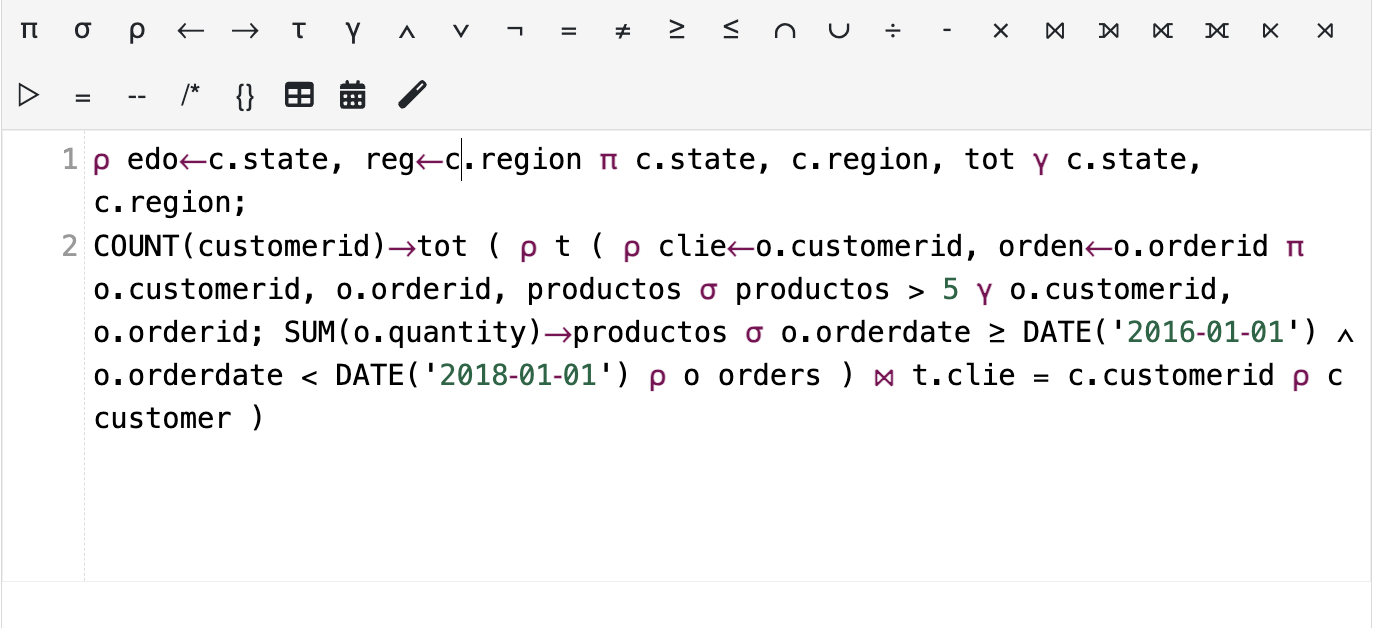
\includegraphics[width=0.8\textwidth]{imagenes/2f(1).png}
\caption{Consulta}
\end{figure}

\begin{figure}[h!]
\centering
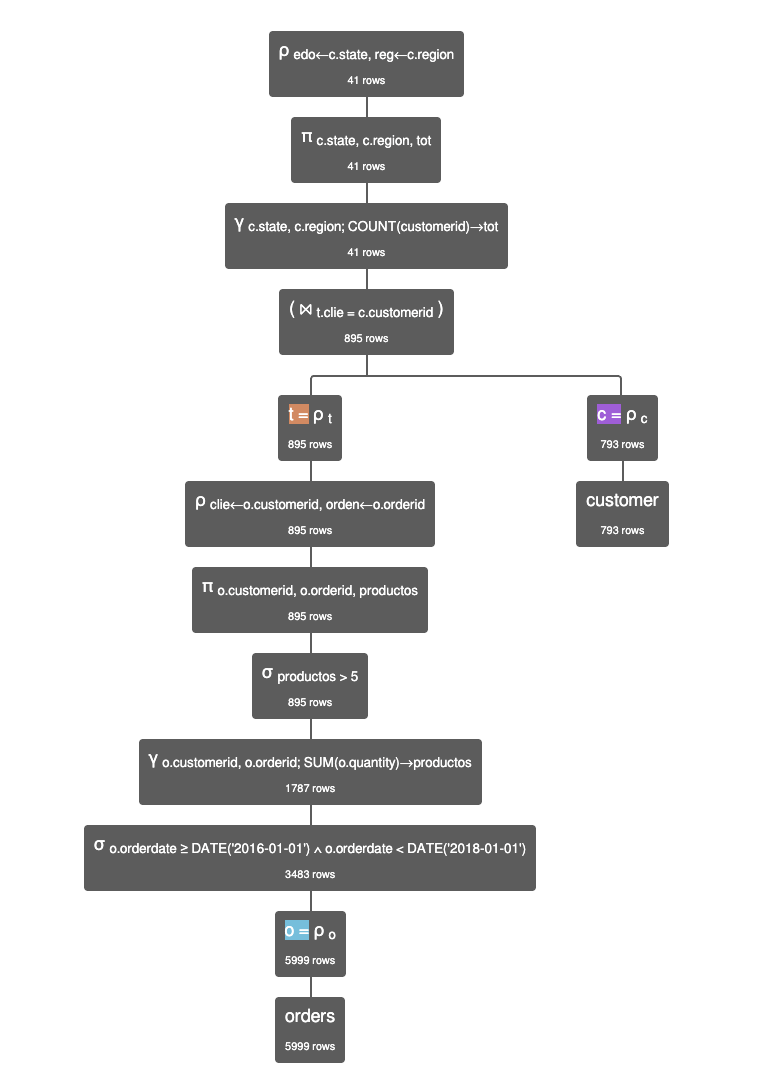
\includegraphics[width=0.8\textwidth]{imagenes/2f(2).png}
\caption{Árbol de consulta.}
\end{figure}

\begin{figure}[h!]
\centering
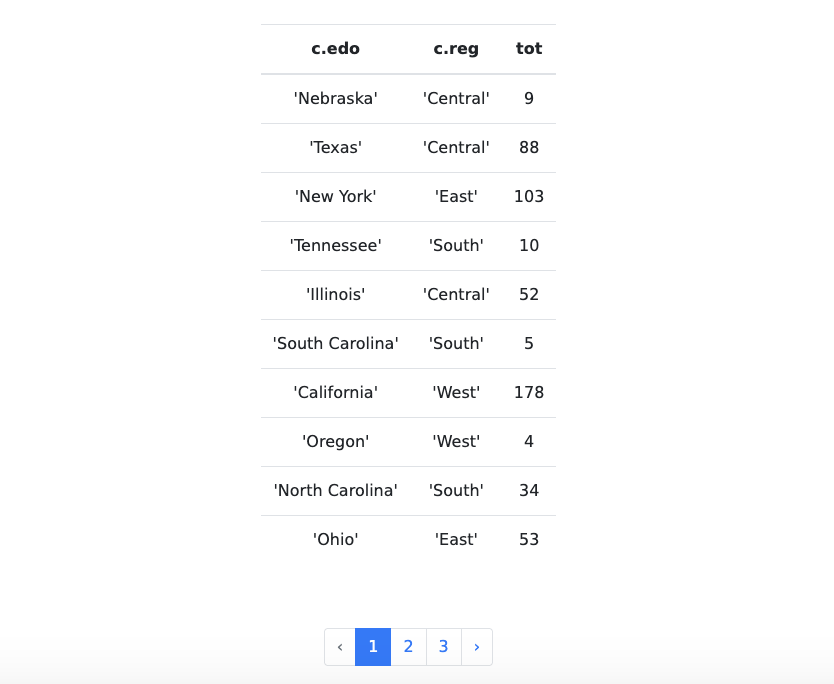
\includegraphics[width=0.6\textwidth]{imagenes/2f(3).png}
\caption{Resultado de consulta.}
\end{figure}